\documentclass[11pt,letterpaper]{article}

% ── Fonts ─────────────────────────────────────────────────────────
\usepackage[T1]{fontenc}
\usepackage{newtxtext}
\usepackage{amssymb}
\usepackage{newtxmath}
\usepackage[scaled=0.85]{inconsolata}

% ── Layout ────────────────────────────────────────────────────────
\usepackage[margin=1in]{geometry}
\usepackage{setspace}
\setstretch{1.08}
\usepackage{parskip}
\setlength{\parskip}{0.5\baselineskip plus 2pt minus 1pt}

% ── Section headings ──────────────────────────────────────────────
\usepackage{titlesec}
\titleformat{\section}{\large\bfseries}{\thesection}{1em}{}
\titleformat{\subsection}{\normalsize\bfseries}{\thesubsection}{0.8em}{}
\titleformat{\subsubsection}{\normalsize\itshape}{\thesubsubsection}{0.8em}{}
\titlespacing*{\section}{0pt}{1.8ex plus 0.5ex}{0.8ex plus 0.2ex}
\titlespacing*{\subsection}{0pt}{1.4ex plus 0.3ex}{0.4ex plus 0.1ex}

% ── Math ──────────────────────────────────────────────────────────
\usepackage{amsmath}
\usepackage{mathtools}

% ── Tables ────────────────────────────────────────────────────────
\usepackage{booktabs}
\usepackage{array}
\usepackage{tabularx}
\renewcommand{\arraystretch}{1.15}
\usepackage{caption}
\captionsetup{font=small, labelfont=bf, labelsep=period, skip=6pt}
\captionsetup[table]{position=above}

% ── Floats ───────────────────────────────────────────────────────
\usepackage{float}
\usepackage{graphicx}
\usepackage{placeins}  % for \FloatBarrier
\graphicspath{{../experiments/analysis/figures/}}
\setlength{\floatsep}{6pt plus 2pt minus 2pt}
\setlength{\textfloatsep}{8pt plus 2pt minus 2pt}
\setlength{\intextsep}{6pt plus 2pt minus 2pt}

% ── Lists ─────────────────────────────────────────────────────────
\usepackage{enumitem}
\setlist{nosep, leftmargin=1.5em}

% ── Colors & Links ────────────────────────────────────────────────
\usepackage{xcolor}
\definecolor{linkblue}{HTML}{0B5394}
\definecolor{citegreen}{HTML}{1B7340}
\definecolor{urlgray}{HTML}{444444}

% ── TikZ (diagrams) ──────────────────────────────────────────────
\usepackage{tikz}
\usetikzlibrary{arrows.meta, positioning, shapes.geometric, calc}

\usepackage[
  colorlinks=true,
  linkcolor=linkblue,
  citecolor=citegreen,
  urlcolor=urlgray,
  bookmarksnumbered=true,
  pdfstartview=FitH,
]{hyperref}
\usepackage[noabbrev,capitalise]{cleveref}

% ── Microtypography ──────────────────────────────────────────────
\usepackage{microtype}

% ── Custom commands ──────────────────────────────────────────────
\newcommand{\pval}[1]{\ensuremath{p = #1}}
\newcommand{\oracle}[1]{\textsc{#1}}
\newcommand{\baseline}{\oracle{Baseline}}
\newcommand{\shifted}{\oracle{Shifted}}
\newcommand{\rewired}{\oracle{Rewired}}
\newcommand{\noisy}{\oracle{Noisy}}

% ══════════════════════════════════════════════════════════════════
\title{\textbf{Structured Reasoning in LLM Optimization Agents:\\[2pt]
  Scaffolding, Not Regularization}}
\author{Kartik G Bhat\thanks{Independent Researcher. Contact:
  \texttt{gkartik@gmail.com}. Code and data:
  \url{https://github.com/kar-ganap/synthoracle}.}}
\date{}

\begin{document}
\maketitle

% ══════════════════════════════════════════════════════════════════
\begin{abstract}\noindent
LLM-based optimization agents increasingly produce structured reasoning
artifacts---hypothesis summaries, causal models, prediction logs---that
persist across iterations. The assumption is that forcing
articulation regularizes reasoning, as the self-explanation effect
suggests it does for human learners. We
test this assumption using SynthOracle, a family of synthetic
multi-objective optimization oracles with known causal structure that
enables separate measurement of optimization quality and reasoning
quality. We pair the benchmark with a verbal regularization (VR)
protocol that requires the agent to hypothesize, predict, and reconcile
at each iteration via a structured summary embedded in conversation
context. Through controlled ablations on two oracles and two models
(Claude Opus~4.6 and Sonnet~4.6; $n = 5$ paired seeds per condition),
we find that the forced summary is
\emph{scaffolding}, not regularization: it improves optimization for a
less capable model (Sonnet, $+26\%$) and a harder task (12-dimensional
with noise, $+14\%$ to $+35\%$), but \emph{hurts} the most capable
model on the simplest oracle (Opus, $-35\%$, \pval{0.0006}). The
pattern is consistent across 18 of 20 paired seeds (binomial
\pval{0.0002}). A mechanism-isolation experiment shows that the
performance penalty comes from the summary's \emph{persistence} in conversation context, not
from the cognitive cost of producing it: an agent that produces the
summary but does not receive it back performs identically to one that
never produces it (\pval{0.35}). We connect this finding to the
architectural trend in frontier reasoning models toward ephemeral
chain-of-thought traces and derive a design principle: match the rigidity
of your reasoning protocol to the gap between model capability and task
difficulty.
\end{abstract}

% ══════════════════════════════════════════════════════════════════
\section{Introduction}
\label{sec:intro}

Large language models (LLMs) are increasingly deployed as autonomous
agents for scientific optimization---selecting experiments, forming hypotheses, and
iterating toward optimal designs. Recent systems pair LLMs with Bayesian
optimization (BO) \cite{cisse2025bora}, embed them in closed-loop experimental
workflows \cite{boiko2023autonomous}, or use them as surrogate-guided
searchers \cite{ramos2024bayesian}. A common design choice across these
systems \cite{cisse2025bora, boiko2023autonomous} is to require the
agent to produce structured reasoning artifacts: chain-of-thought
traces, hypothesis summaries, or causal model descriptions that persist
across iterations.

The assumption behind this choice borrows from human cognition. The
self-explanation effect \cite{chi1994selfexplanation} demonstrates that
articulating understanding improves learning: students who explain
material to themselves acquire deeper knowledge than those who do not.
For human scientists, writing down a model forces coherence and exposes
gaps---a form of cognitive regularization.

Yet rigorous evidence for this assumption in LLM agents is thin. Gupta
et~al.\ \cite{gupta2025arewethereyet} showed that BioDiscoveryAgent,
despite producing ``Reflection'' and ``Research Plan'' text at each
iteration, exhibits zero sensitivity to whether experimental feedback is
real or permuted---suggesting the reasoning text is decorative. BORA
\cite{cisse2025bora} demonstrated that LLM-generated hypotheses improve
Bayesian optimization, but the hypotheses are correlational, not causal,
and the system does not verify whether the LLM actually updates its
beliefs from data. Neither system can measure reasoning quality
independently of optimization quality, because neither has access to
ground-truth causal structure.

This measurement gap is the starting point for our work. Without ground
truth, one cannot distinguish an agent that optimizes well because it
understood the system from one that optimizes well despite misunderstanding
it. To close this gap, we introduce \textbf{SynthOracle}, a family of
synthetic multi-objective optimization oracles with known causal
structure. Each oracle defines a directed acyclic graph (DAG) from inputs
through mechanisms to outputs, with functional forms composed of standard
building blocks (sigmoid, exponential, power law) in non-standard
combinations designed to be unlikely to appear in LLM training
data. The benchmark enables separate measurement of optimization quality
(hypervolume relative to Bayesian optimization) and reasoning quality
(precision and recall of discovered causal edges against the ground-truth
DAG).

We pair the benchmark with a \emph{verbal regularization} (VR) protocol:
the agent iteratively hypothesizes causal relationships, makes
quantitative predictions, reconciles prediction errors with observations,
and produces a structured iteration summary---a schema-parsed object
specifying claimed edges, confidence scores, surprises, and
next-iteration plans. This summary is embedded in the condensed
conversation context that persists across iterations, serving as the
agent's articulated causal model.

Our central finding contradicts the regularization assumption. Through a
series of controlled ablations on two oracles (\baseline{}: 6 inputs, all
relevant; \noisy{}: 12 inputs, 6 irrelevant) and two models (Opus,
Sonnet), we show:

\begin{enumerate}
  \item \textbf{The forced summary is scaffolding, not regularization.}
  It helps when the agent needs structure---a less capable model (Sonnet)
  or a harder task (\noisy{}, where screening irrelevant dimensions
  benefits from articulated beliefs). It hurts when the agent does not
  need it---the most capable model (Opus) on the simplest oracle
  (\baseline{}), where it reduces optimization quality by 35\% (paired
  $t$-test, \pval{0.0006}, $n = 5$). Across all four model--oracle
  combinations, 18 of 20 paired seeds follow the predicted direction
  (binomial \pval{0.0002}).

  \item \textbf{The mechanism is context cementing, not cognitive cost.}
  An agent that produces the structured summary but does not receive it
  back in subsequent context performs identically to one that never
  produces it (paired $t$-test, \pval{0.35}, $n = 5$). Both outperform the
  full VR agent (\pval{0.002}). The act of articulation is free; the
  persistence of articulated beliefs in conversation context cements
  early---often wrong---causal claims into subsequent reasoning.

  \item \textbf{The agent genuinely learns from data.} A
  permuted-feedback ablation shows 66\% higher optimization quality with
  real versus scrambled feedback, contradicting the finding of Gupta
  et~al.\ \cite{gupta2025arewethereyet} in the continuous-structured
  setting. Per-iteration surprise counts decrease monotonically across
  both oracles ($n = 5$, 144 evaluations).
\end{enumerate}

These findings yield a design principle for practitioners building LLM
optimization agents: match the rigidity of your reasoning protocol to the
gap between your model's capability and your task's difficulty. The
context-cementing mechanism also connects to a broader architectural
pattern in frontier reasoning models, where chain-of-thought traces are
produced but kept ephemeral rather than persisted in conversation
context---a design choice consistent with the mechanism we identify.

The remainder of this paper is organized as follows.
\Cref{sec:related} reviews related work.
\Cref{sec:benchmark} introduces the SynthOracle benchmark.
\Cref{sec:protocol} describes the verbal regularization protocol.
\Cref{sec:experiments} presents experimental results.
\Cref{sec:discussion} discusses implications and limitations.
\Cref{sec:conclusion} concludes.


% ══════════════════════════════════════════════════════════════════
\section{Related Work}
\label{sec:related}

Our work intersects three lines of research: LLM-assisted optimization,
feedback sensitivity in LLM agents, and interpretable intermediate
representations.

\subsection{LLM-assisted optimization}

Several recent systems integrate LLMs into optimization loops. BORA
\cite{cisse2025bora} defines an adaptive three-action policy: vanilla
Bayesian optimization when the Gaussian process (GP) is confident,
LLM-generated candidates when it is uncertain, and a collaborative mode
at intermediate uncertainty. The system outperforms five baselines on
mixed synthetic and chemistry benchmarks, demonstrating that LLM priors
accelerate early-stage search. However, BORA's LLM hypotheses are
correlational (``increasing temperature improves yield''), not
mechanistic, and the system does not track whether the LLM updates its
beliefs from experimental outcomes. Boiko et~al.\
\cite{boiko2023autonomous} deploy an LLM agent for autonomous chemical
synthesis with tool access, demonstrating multi-step planning, but
without controlled comparison to non-LLM baselines or measurement of
reasoning quality.

Our work differs in two respects. First, we require the agent to
articulate \emph{causal} hypotheses---directed edges with confidence
scores---rather than correlational statements, enabling measurement of
reasoning quality via edge precision and recall against ground truth.
Second, we ablate the reasoning protocol itself, isolating whether
structured articulation helps or hurts, rather than comparing
LLM-assisted optimization to LLM-free optimization.

\subsection{Feedback sensitivity in LLM agents}

Gupta et~al.\ \cite{gupta2025arewethereyet} introduced a
permuted-feedback ablation for LLM experimental-design agents: scramble
the mapping between candidate selections and observed outcomes while
preserving marginal distributions. Applied to BioDiscoveryAgent on
discrete library-selection tasks, the ablation revealed zero feedback
sensitivity---the agent performs equally well with real and fake
outcomes. The authors conclude that LLM value derives entirely from
priors (domain knowledge encoded during pre-training), not from
posterior updating on experimental data. Their proposed alternative,
LLMNN (LLM Nearest Neighbor), separates the LLM's role into seed-point
generation (priors only) and nearest-neighbor expansion (classical
methods).

Our setting differs in three structural ways that may explain the
divergent result. First, our oracle is continuous (6--12 real-valued
inputs) rather than discrete (library selection), providing richer
gradient information. Second, our protocol requires \emph{quantitative
predictions} before each evaluation, creating an explicit
prediction-error signal the agent must reconcile. Third, our oracle has
mechanistic structure (interacting mechanisms, thresholds, regime
transitions) that rewards systematic exploration over random sampling.
Under these conditions, we observe strong feedback sensitivity: 66\%
higher hypervolume with real versus permuted feedback.

\subsection{Concept bottleneck models}

Concept bottleneck models (CBMs) \cite{koh2020cbm} force a neural
network to route predictions through a layer of human-interpretable
concepts before producing outputs. When the concepts are correct and
sufficient, the bottleneck regularizes the model by preventing reliance
on spurious features. When concepts are wrong or incomplete, the
bottleneck constrains the model to an incorrect intermediate
representation, degrading performance \cite{yuksekgonul2023posthoc}.

Our structured iteration summary functions as a \emph{learned} concept
bottleneck: the agent constructs its own interpretable intermediate
representation (claimed causal edges with confidence scores) that
mediates between raw observations and optimization decisions. The key
difference from standard CBMs is that the bottleneck is not designed by
the researcher but discovered by the agent---and its quality depends on
the agent's capability and the task's difficulty. Our 2$\times$2 matrix
(\cref{sec:experiments}) empirically confirms the CBM prediction: the
bottleneck helps when concepts are correct (screening noise dimensions on
\noisy{}) and hurts when early concepts are wrong (threshold effects on
\baseline{}).

\subsection{Chain-of-thought and structured reasoning}

Chain-of-thought prompting \cite{wei2022chainofthought} and ReAct
\cite{yao2023react} demonstrate that eliciting intermediate reasoning
steps improves LLM performance on single-turn tasks. Our work examines a
different question: what happens when structured reasoning artifacts
\emph{persist across turns} in a multi-iteration agent loop? The
distinction matters because persistence creates a commitment device---the
agent's prior reasoning anchors subsequent iterations---which can be
beneficial (maintaining useful beliefs) or harmful (cementing wrong ones).
This is orthogonal to the single-turn finding that reasoning steps help:
producing a chain of thought within one iteration may be universally
beneficial, but carrying it forward into the next iteration's context is
not.

% ══════════════════════════════════════════════════════════════════
\section{SynthOracle Benchmark}
\label{sec:benchmark}

SynthOracle is a family of synthetic multi-objective optimization oracles
designed to evaluate whether LLM agents learn causal structure, not just
find good solutions. Each oracle is a deterministic Python function
$f: \mathbb{R}^d \to \mathbb{R}^4$ mapping $d$ inputs to four outputs
with mixed optimization directions (maximize $Y_1$, minimize $Y_2$,
threshold $Y_3 > 0.4$, maximize $Y_4$). Evaluations take $<$1\,ms and
require no API calls, enabling high-throughput experimentation at zero
marginal cost.

\subsection{Oracle family}

The benchmark comprises four oracles that share a common mechanism
topology but vary along independent structural axes
(\cref{fig:oracle_dags}, \cref{tab:oracle_properties}). All four route
inputs through four intermediate mechanisms ($M_1$--$M_4$: throughput,
leakage, coupling, and threshold gating) before producing outputs. The
functional forms combine standard building blocks---sigmoid activations,
exponential decay, power laws, rational functions---in non-standard
compositions unlikely to appear in LLM training corpora. Full equations
and parameter values are provided in \cref{app:oracle_specs}.

\begin{figure}[htbp]
\centering
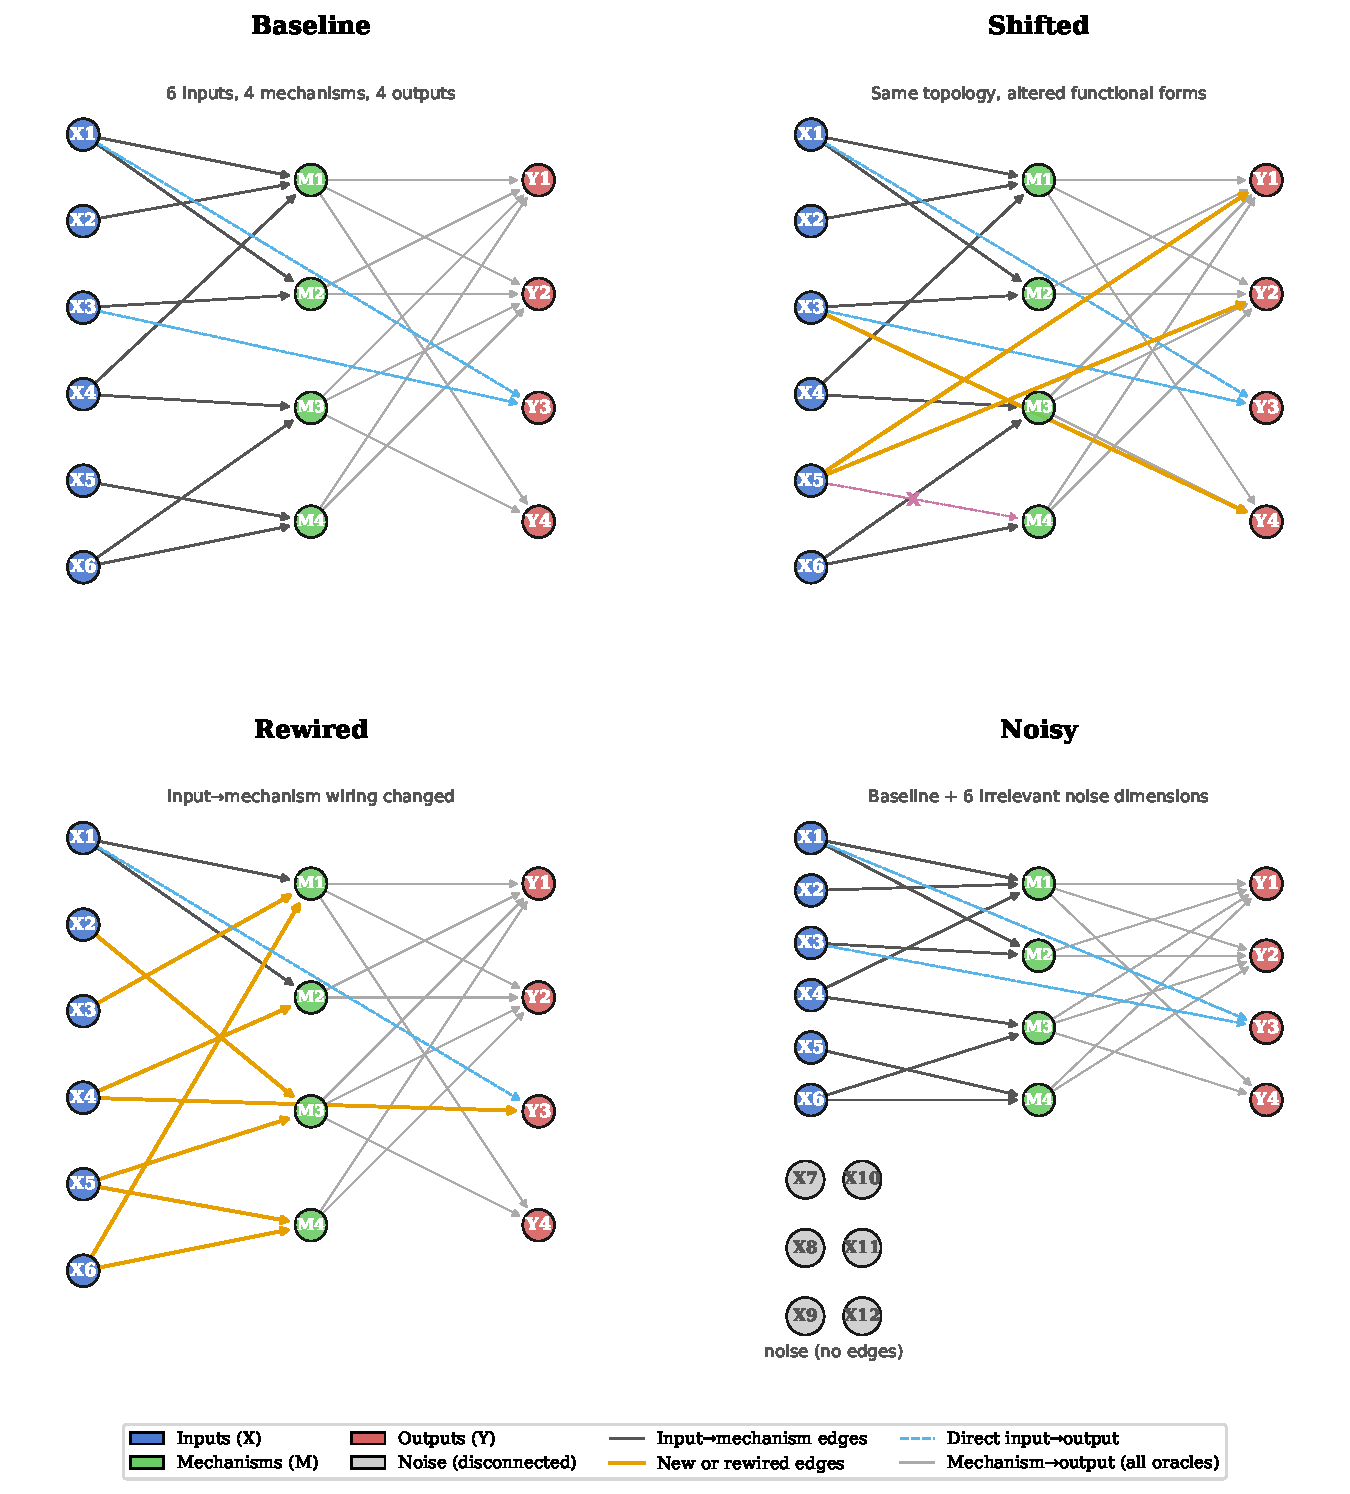
\includegraphics[width=\textwidth]{fig1_oracle_dags.pdf}
\caption{Causal structure of the four SynthOracle oracles. Inputs
  (blue) connect to mechanisms (green) which produce outputs (red).
  Dark arrows: shared edges. Orange arrows: new or rewired edges
  relative to \baseline{}. Dashed blue: direct input--output paths.
  Gray nodes in \noisy{}: disconnected noise dimensions.
  Mechanism--output edges (light gray) are shared across all oracles.}
\label{fig:oracle_dags}
\end{figure}

\paragraph{\baseline{}} The reference oracle. Six inputs, all causally
relevant, with 26 mechanism-level edges (18 when projected to
input--output pairs). Features include a regime transition at $X_1
\approx 0.27$, a hidden coupling intermediate ($M_3 = X_4 / (X_4 +
X_6)$) that modulates two mechanisms, and a sharp threshold activation
at $X_5 = 0.38$.

\paragraph{\shifted{}} Same mechanism topology as \baseline{}, but with
altered functional forms: the threshold is disabled (gate $\equiv 1$), a
monotonic relationship becomes inverted-U, and an output sign is flipped.
Tests whether an agent can \emph{unlearn} incorrect functional-form
assumptions when the causal graph is preserved.

\paragraph{\rewired{}} Same number of mechanisms but with input--mechanism
wiring swapped: the inputs that drove throughput ($M_1$) in \baseline{}
now drive leakage ($M_2$) and vice versa. Tests whether an agent can
\emph{dismiss} prior structural beliefs when the topology changes.
Transfer experiments using \shifted{} and \rewired{} are reported in
\cref{app:transfer}.

\paragraph{\noisy{}} Identical to \baseline{} but embedded in a
12-dimensional input space: the six real inputs ($X_1$--$X_6$) retain
their causal effects; six noise inputs ($X_7$--$X_{12}$) have zero
effect on all outputs. Tests the agent's ability to \emph{screen}
irrelevant dimensions. The mechanism-to-input ratio drops from
$k/d = 1.17$ (\baseline{}) to $k/d = 0.58$: an agent that identifies
the 6 noise inputs via causal reasoning effectively reduces its search
space from 12 to 6 dimensions, while BO's Gaussian process must model
all 12.

% ── Table 1: Oracle properties ──
\begin{table}[t]
\centering
\caption{Oracle intrinsic properties. $d$: input dimensionality.
$k$: number of mechanisms. $R^2(M \!\to\! Y)$: fraction of output
variance explained by mechanism activations (mean across outputs).
IO edges: number of input--output (IO) edges in the projected
ground-truth DAG.}
\label{tab:oracle_properties}
\small
\begin{tabular}{@{}lccccccl@{}}
\toprule
Oracle & $d$ & $k$ & $k/d$ & $R^2(M\!\to\!Y)$ & IO edges & Noise dims
  & What varies vs.\ \baseline{} \\
\midrule
\baseline{} & 6 & 7 & 1.17 & 0.961 & 18 & 0 & Reference \\
\shifted{}  & 6 & 7 & 1.17 & 0.748 & 19 & 0 & Functional forms \\
\rewired{}  & 6 & 7 & 1.17 & 0.960 & 19 & 0 & Input--mechanism wiring \\
\noisy{}    & 12 & 7 & 0.58 & 0.961 & 18 & 6 & 6 irrelevant dimensions \\
\bottomrule
\end{tabular}
\end{table}

\subsection{Diagnostic suite}
\label{sec:diagnostics}

The key property of SynthOracle is that each oracle's ground-truth DAG
is known, enabling measurement of reasoning quality independently of
optimization quality. We define four diagnostic metrics.

\paragraph{Edge precision and recall.} The ground-truth DAG contains
mechanism-level edges (e.g., $X_1 \!\to\! M_1 \!\to\! Y_1$). The
IO projection collapses these by tracing reachability:
if any path exists from $X_i$ to $Y_j$ through mechanisms, the edge
$X_i \!\to\! Y_j$ is included. The agent's discovered edges are
compared against this projected DAG. An edge is counted as discovered if, when replaying the
agent's one-at-a-time (OAT) sweeps on the oracle, the output range
exceeds a threshold of 0.05 (5\% of output scale). Precision measures
the fraction of claimed edges that are real; recall measures the fraction
of real edges that are found. Sensitivity analysis confirms that
precision is 1.00 for all thresholds tested (0.01--0.20) due to complete
separation between true-edge and noise-edge effect sizes
(\cref{app:threshold_sensitivity}).

\paragraph{Screening efficiency.} On \noisy{}, we measure the fraction
of OAT sweeps directed at noise inputs and the maximum confidence
assigned to any noise edge in the agent's final iteration summary. An
agent with perfect screening spends zero evaluation budget on noise
dimensions and assigns zero confidence to noise edges.

\paragraph{Calibration learning.} At fixed evaluation counts, the agent
is asked to predict outputs for a held-out test point. The mean absolute
error (MAE) between predicted and actual outputs measures prediction
quality. A decrease in MAE from the first to last calibration checkpoint
indicates the agent's internal model is improving.

\paragraph{Surprise trajectory.} At each iteration, the agent reports
events that contradicted its current model. A decreasing surprise count
indicates the agent is updating its beliefs to match the data.

The benchmark additionally provides Sobol-weighted information capture,
OAT prediction accuracy, sample efficiency curves, and adversarial
region error; these are reported in \cref{app:additional_diagnostics}.

\subsection{Bayesian optimization baseline}

We compare VR against multi-objective Bayesian optimization using
qNEHVI \cite{daulton2021nehvi} with a standard Gaussian process
surrogate, implemented in BoTorch. Both methods receive the same
Latin Hypercube Sampling (LHS) initialization ($2d$ points). BO runs
use batch size 1 with sequential acquisition. We report hypervolume
(HV) as the primary optimization metric, computed against a reference
point derived from the oracle's output ranges.

% ══════════════════════════════════════════════════════════════════
\section{Verbal Regularization Protocol}
\label{sec:protocol}

The VR agent is an LLM-driven optimization loop
that interleaves oracle evaluations with structured causal reasoning. The
agent receives a system prompt describing the oracle's inputs, outputs,
optimization directions, and the feasibility constraint $Y_3 > 0.4$
(designs violating this constraint are infeasible), but no information
about the underlying mechanism structure. It iterates until
the evaluation budget is exhausted.

\subsection{Tool suite}

The agent interacts with the oracle through two categories of tools.

\paragraph{Evaluation tools} consume budget (one oracle call each):
\begin{itemize}
  \item \emph{Point evaluation}: evaluate the oracle at a specific input
  vector; returns outputs and prediction errors (if the agent provided
  predictions).
  \item \emph{OAT sweep}: one-at-a-time sensitivity sweep---vary one
  input across its range while holding others fixed; returns output
  trajectories and predicted-vs-actual trend comparisons.
  \item \emph{Interaction test}: $2 \times n$ factorial design for two
  inputs; returns interaction effect sizes.
\end{itemize}

\paragraph{Analysis tools} are free (computed from existing data):
pairwise correlation matrix, input sensitivity estimates, local
finite-difference gradients, current Pareto front with hypervolume, and
linear regression fits. These allow the agent to analyze accumulated
data without spending evaluation budget.

The tool design embodies the VR principle: evaluation tools require the
agent to make \emph{quantitative predictions} before observing results.
For point evaluations, the agent predicts output values; for OAT
sweeps, it predicts monotonic trend directions. Prediction
errors are returned alongside actual values, creating an explicit
reconciliation signal.

\subsection{Iteration loop}

Each iteration proceeds as follows:

\begin{enumerate}
  \item The agent receives a condensed context containing: the current
  evaluation count and budget remaining, output value ranges observed so
  far, the most recent evaluation results, and (if
  summary generation is enabled) the agent's prior
  structured summary under a heading ``Your Causal Model.''
  \item The agent makes up to 15 tool calls per iteration, freely
  choosing which tools to invoke and in what order.
  \item After tool calls complete, the agent produces a \emph{structured
  iteration summary}: a structured object parsed against a fixed schema,
  containing:
  \begin{itemize}
    \item \emph{Edges}: a list of claimed causal edges, each with a
    source, target, confidence score (0--1), and brief rationale;
    \item \emph{Surprises}: observations that contradicted the agent's
    current model;
    \item \emph{Findings}: mechanistic insights gained this iteration;
    \item \emph{Plan}: what the agent intends to investigate next.
  \end{itemize}
  \item At configurable intervals (every 20 evaluations by default), a
  \emph{calibration checkpoint} asks the agent to predict outputs for a
  random held-out input, measuring prediction quality over time.
\end{enumerate}

Between iterations, the conversation is condensed: the full tool-call
history is replaced with a compact status message, preserving the
structured summary as persistent context. This condensation is necessary
because multi-iteration runs with 15 tool calls per iteration would
otherwise exceed the model's context window. It is also the mechanism
through which the structured summary \emph{cements} into subsequent
reasoning---the ablation target in our experiments.

\subsection{Ablation parameters}

The protocol exposes two boolean parameters that enable the controlled
ablations reported in \cref{sec:experiments}:

\begin{itemize}
  \item \emph{Skip summary}: the agent does not produce the structured
  summary. It retains access to all tools and makes the same number of
  tool calls, but no iteration summary is generated or persisted.
  \item \emph{Summary not in context}: the agent produces the structured
  summary (which is logged for analysis), but the summary is \emph{not}
  embedded in the condensed context for the next iteration. The agent
  receives a generic status message instead of its prior causal model.
\end{itemize}

These two parameters create a clean three-condition experimental design:
(1)~summary produced and in context (full VR), (2)~summary produced but
not in context, and (3)~no summary produced. Comparing conditions 1
vs.~2 isolates the effect of \emph{persistence}; comparing 2 vs.~3
isolates the effect of \emph{articulation}.

\subsection{Implementation}

All experiments use the Anthropic Messages API with adaptive extended
thinking (\cref{app:prompt} provides the full prompt template and output
schema). The default model is Claude Opus~4.6; model-comparison
experiments additionally use Sonnet~4.6 and Haiku~4.5. Maximum output
tokens are set to 16{,}000 (24{,}000 for 144-evaluation extended runs).
Latin Hypercube Sampling provides $2d$ initial points (12 for \baseline{},
24 for \noisy{}) shared across VR and BO conditions for each seed.

% ══════════════════════════════════════════════════════════════════
\section{Experiments}
\label{sec:experiments}

All VR experiments use $n = 5$ seeds (42--46) and all BO experiments use
$n = 3$ seeds (42--44) unless otherwise noted. BO's lower seed count
reflects its lower variance: the deterministic acquisition function
(qNEHVI) introduces variability only through the LHS initialization.

\subsection{VR pays an understanding tax that scales with $k/d$}
\label{sec:understanding_tax}

\Cref{tab:main_results} summarizes optimization and causal discovery
results; \cref{fig:hv_trajectories} shows the HV trajectories on
\baseline{} and \noisy{} at 144 evaluations.
On \baseline{}, VR reaches 69\% of BO at 72 evaluations and converges to
99\% at 144. On \noisy{}, VR reaches 94\% at 72 evaluations and 98\% at
144. The gap between the two oracles reflects the mechanism-to-input
ratio $k/d$: when irrelevant dimensions outnumber mechanisms
(\noisy{}, $k/d = 0.58$), VR's ability to screen inputs via causal
reasoning provides a structural advantage that partially offsets the
understanding tax.

\begin{figure}[htbp]
\centering
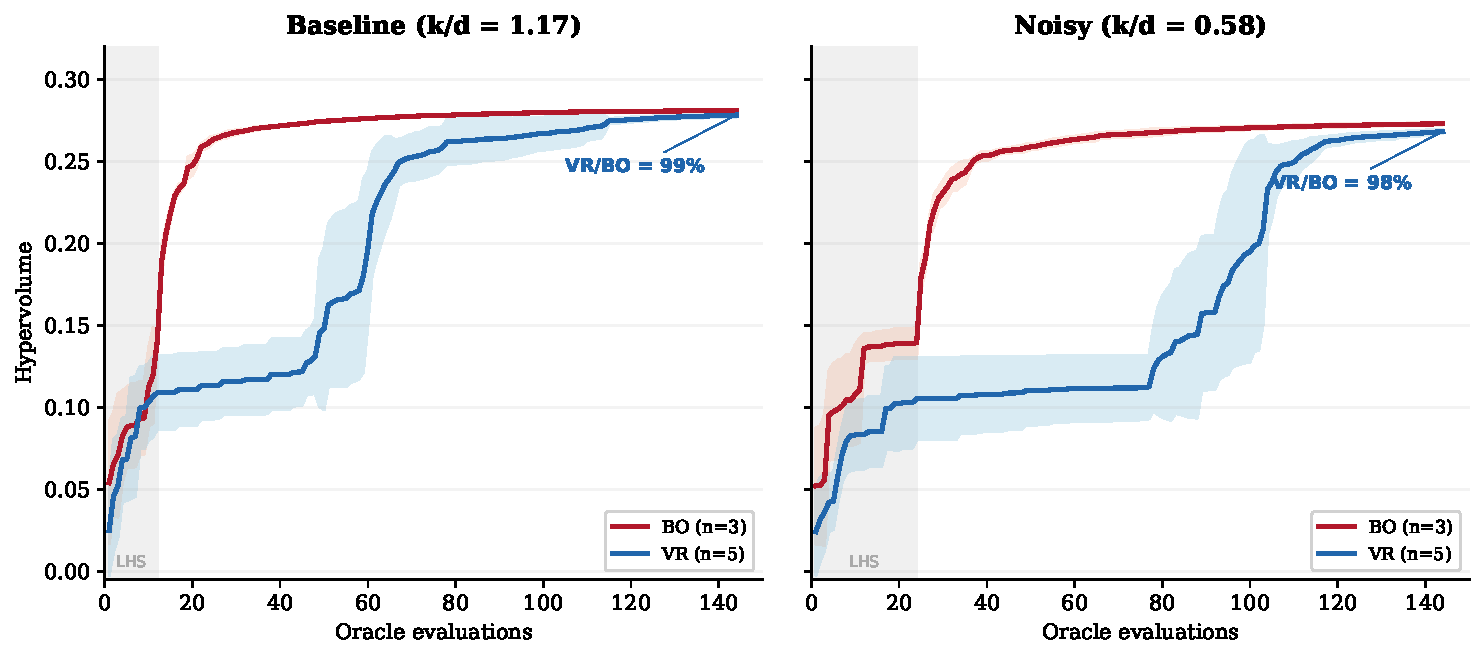
\includegraphics[width=\textwidth]{fig2_hv_trajectories.pdf}
\caption{Hypervolume trajectories on \baseline{} and \noisy{} (144
  evaluations). VR: $n = 5$ seeds (mean $\pm$ 1\,s.d.\ shaded).
  BO: $n = 3$ seeds. Shaded region at left: Latin Hypercube Sampling
  initialization. VR converges to 99\% of BO on \baseline{} and 98\%
  on \noisy{}. On \noisy{}, the agent invests the first ${\sim}80$
  evaluations in model-building (flat HV) before exploiting.}
\label{fig:hv_trajectories}
\end{figure}

Edge precision is 1.00 across all conditions---the agent never claims a
false causal edge. Recall is 0.94 on \baseline{} (the consistently
missed edge is the hidden threshold $X_5 \to Y_2$) and rises from 0.70
at 72 evaluations to 0.94 at 144 on \noisy{}, indicating that extended
budget enables more complete causal discovery.

% ── Table 2: Main results ──
\begin{table}[t]
\centering
\caption{Optimization and causal discovery results. VR: $n = 5$
  seeds. BO: $n = 3$ seeds. Edge precision and recall computed by
  replaying OAT sweeps against the IO-projected ground-truth DAG
  (threshold = 0.05).}
\label{tab:main_results}
\small
\begin{tabular}{@{}llccccc@{}}
\toprule
Oracle & Budget & VR HV & BO HV & VR/BO & Precision & Recall \\
\midrule
\baseline{} & 72  & $.192 \pm .015$ & $.278 \pm .001$ & 69\% & 1.00 & 0.94 \\
             & 144 & $.278 \pm .001$ & $.281 \pm .000$ & 99\% & 1.00 & 0.94 \\
\noisy{}    & 72  & $.251 \pm .017$ & $.267 \pm .001$ & 94\% & 1.00 & 0.70 \\
             & 144 & $.268 \pm .001$ & $.273 \pm .001$ & 98\% & 1.00 & 0.94 \\
\bottomrule
\end{tabular}
\end{table}

\FloatBarrier
\subsection{The agent uses feedback, contra Gupta et al.}
\label{sec:feedback}

We replicate the permuted-feedback ablation of Gupta et~al.\
\cite{gupta2025arewethereyet} on \baseline{}. Two VR runs share the
same LHS initialization (seed~42, 12 points): one receives real oracle
outputs; the other receives outputs with the candidate--outcome mapping
scrambled (preserving marginal distributions). \Cref{fig:permuted}
shows the result: trajectories overlap during LHS and diverge
immediately afterward (evaluation~13). The real-feedback agent reaches
HV~$= 0.219$; the permuted agent plateaus at $0.132$---a 66\%
difference.

\begin{figure}[htbp]
\centering
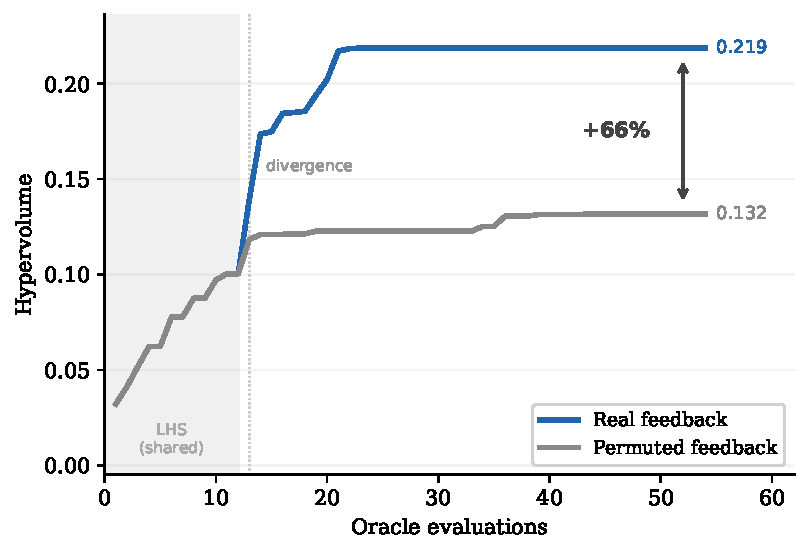
\includegraphics[width=0.55\textwidth]{fig3_permuted_feedback.pdf}
\caption{Permuted-feedback ablation on \baseline{} (seed~42).
  Both conditions share the same LHS initialization (12~points).
  Trajectories diverge at evaluation~13. Real feedback: HV~$= 0.219$.
  Permuted: $0.132$ ($+66\%$ effect).}
\label{fig:permuted}
\end{figure}

This contradicts the finding of Gupta et~al.\ that LLM agents show
zero feedback sensitivity on discrete experimental-design tasks. In
our continuous-structured setting, where the agent makes quantitative
predictions and receives explicit prediction errors, feedback is
load-bearing.

\FloatBarrier
\subsection{The agent's causal model improves over iterations}
\label{sec:learning}

\Cref{fig:learning} shows per-iteration surprise counts for both
oracles at 144 evaluations ($n = 5$ matched seeds). Surprise counts
decrease monotonically from ${\sim}5$ at iteration~1 to ${\sim}2$ at
iteration~4 on both \baseline{} and \noisy{}, indicating the agent
systematically updates its causal model to better match the data. The
decline is consistent across seeds (error bars overlap between oracles),
suggesting the learning dynamic is robust to oracle structure. Surprise
counts do not reach zero---the agent's causal model remains imperfect
(recall~$= 0.94$, not 1.00), and the consistently missed edge
($X_5 \to Y_2$) continues to generate prediction errors.

\begin{figure}[htbp]
\centering
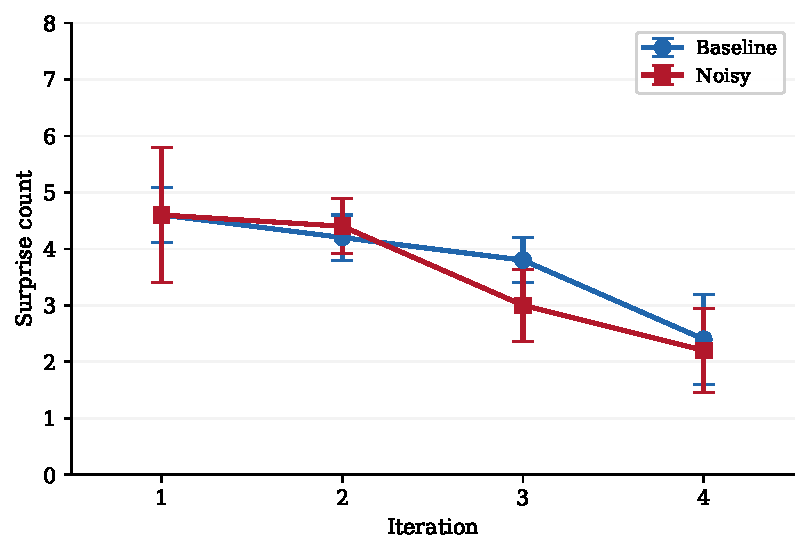
\includegraphics[width=0.55\textwidth]{fig4_learning_trajectories.pdf}
\caption{Per-iteration surprise count on \baseline{} and \noisy{}
  (144 evaluations, $n = 5$ matched seeds 42--46). Both oracles show
  monotonic decline, indicating the agent updates its causal model
  from data. Truncated to 4 iterations (the minimum across all seeds
  in both conditions). Error bars: $\pm$1\,s.d.}
\label{fig:learning}
\end{figure}

\FloatBarrier
\subsection{Forced summaries are scaffolding, not regularization}
\label{sec:scaffolding}

We ablate the structured iteration summary across two models (Opus~4.6,
Sonnet~4.6) and two oracles (\baseline{}, \noisy{}), creating a
$2 \times 2$ matrix of paired comparisons ($n = 5$ seeds per cell).
For each seed, the ``with summary'' and ``without summary'' conditions
share the same LHS initialization, isolating the summary's effect.

\Cref{tab:ablation} and \cref{fig:matrix} present the results. The
summary hurts in exactly one cell: Opus on \baseline{} ($-35\%$,
\pval{0.0006}). In the other three cells, the summary helps: Sonnet on
\baseline{} ($+26\%$, \pval{0.054}), Opus on \noisy{} ($+14\%$,
\pval{0.095}), and Sonnet on \noisy{} ($+21\%$, \pval{0.169}). While
individual $p$-values for the $n = 5$ cells vary, 18 of 20 paired seeds
across all four cells follow the predicted direction (binomial
\pval{0.0002}).

% ── Table 3: Ablation matrix ──
\begin{table}[t]
\centering
\caption{Summary ablation: $2 \times 2$ matrix. $n = 5$ paired seeds
  per cell (seeds 42--46). Effect: percentage change in mean HV due to
  adding the summary. $p$-values from paired $t$-tests.}
\label{tab:ablation}
\small
\begin{tabular}{@{}lccccr@{}}
\toprule
Cell & With summary & Without & Effect & $p$ & Dir.\ \\
\midrule
Opus $\times$ \baseline{}
  & $.192 \pm .015$ & $.259 \pm .014$ & $-35\%$ & $0.0006$ & 5/5 \\
Sonnet $\times$ \baseline{}
  & $.258 \pm .013$ & $.204 \pm .041$ & $+26\%$ & $0.054$ & 5/5 \\
Opus $\times$ \noisy{}
  & $.251 \pm .017$ & $.219 \pm .042$ & $+14\%$ & $0.095$ & 4/5 \\
Sonnet $\times$ \noisy{}
  & $.243 \pm .020$ & $.202 \pm .034$ & $+21\%$ & $0.169$ & 4/5 \\
\midrule
\multicolumn{5}{@{}l}{Global sign consistency: 18/20 seeds}
  & \pval{0.0002} \\
\bottomrule
\end{tabular}
\end{table}

\begin{figure}[htbp]
\centering
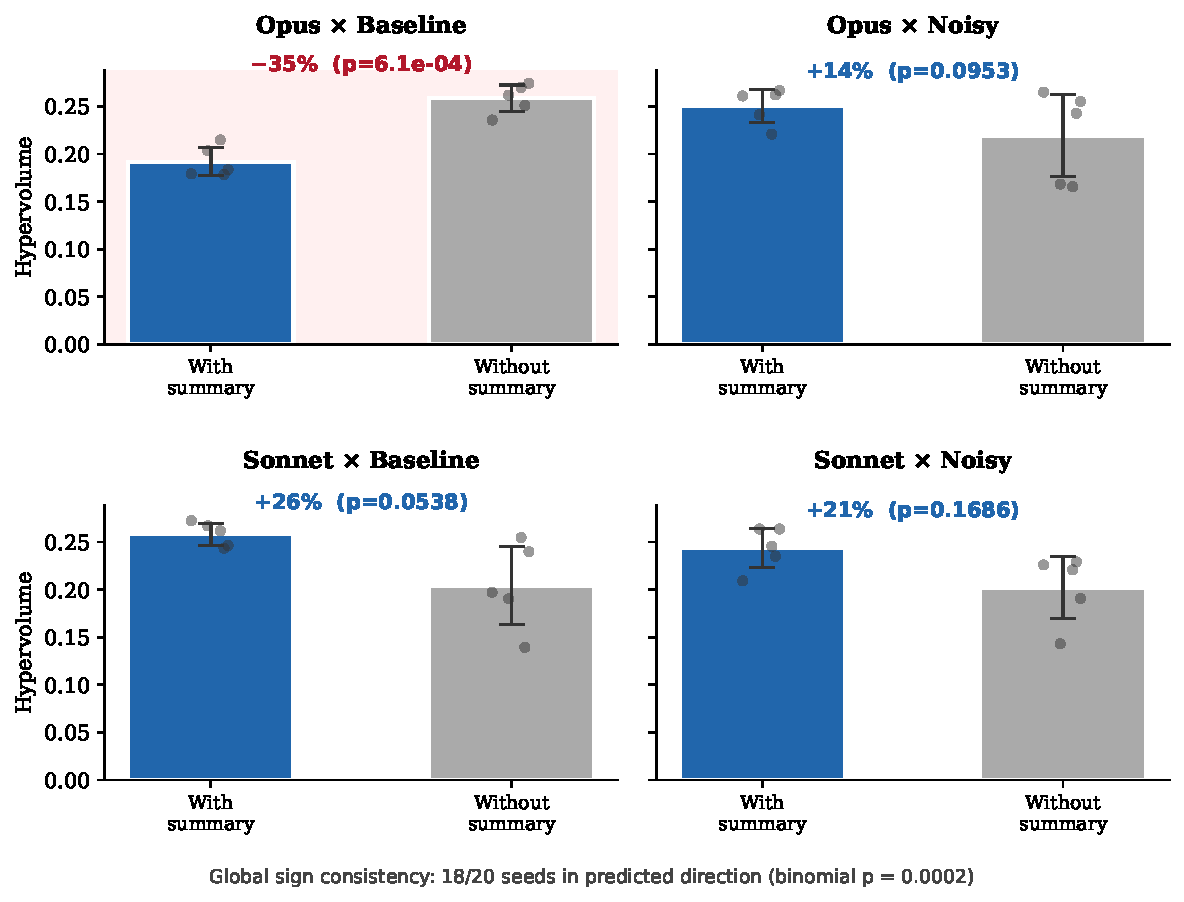
\includegraphics[width=\textwidth]{fig5_2x2_matrix.pdf}
\caption{Summary ablation: $2 \times 2$ matrix. Each panel shows
  mean HV with and without the structured summary ($n = 5$ paired
  seeds). Error bars: $\pm$1\,s.d. Dots: individual seeds. Pink
  background: the one cell where the summary hurts. The summary helps
  in 3 of 4 cells; it hurts only for the most capable model on the
  simplest oracle.}
\label{fig:matrix}
\end{figure}

The pattern admits a clean interpretation: the summary is
\emph{scaffolding}, not regularization. It helps when the agent needs
structure---a less capable model (Sonnet benefits on both oracles) or a
harder task (both models benefit on \noisy{}, where screening noise
dimensions requires systematic tracking of which inputs matter). It
hurts only in the one cell where the agent does not need structure: the
most capable model (Opus) on the simplest oracle (\baseline{}, where all
inputs are relevant and no screening is needed).

Without the summary, raw tool-use capability reveals a 35\% model gap on
\baseline{}: Opus reaches $0.259$, Sonnet only $0.204$. The summary
lifts Sonnet to $0.258$---near parity with unscaffolded Opus---but drags
Opus down to $0.192$. The summary equalizes performance by helping the
weaker model and constraining the stronger one.

This finding also clarifies the ``understanding tax'' reported in
\cref{sec:understanding_tax}. On \baseline{} at 72 evaluations, VR with
the summary reaches 69\% of BO, while VR without the summary reaches
92\%. The total 31-percentage-point gap between VR-with-summary and BO
decomposes as: $100\% - 92\% = 8$ percentage points from VR's
exploration overhead (OAT sweeps, interaction tests versus BO's GP-based
acquisition), and $92\% - 69\% = 23$ percentage points from the summary
cementing early beliefs. On \baseline{}, the summary accounts for
roughly three-quarters of the understanding tax. On \noisy{}, where the
summary aids screening, both components shrink and VR approaches BO
parity. The understanding tax and the scaffolding finding address
different questions: the former asks whether VR is worth using at all
(the answer depends on whether causal understanding is valued alongside
optimization); the latter asks how to configure VR once adopted (match
summary rigidity to the model--task capability gap).

\FloatBarrier
\subsection{The penalty is from persistence, not articulation}
\label{sec:mechanism}

We run a third condition on \baseline{} with Opus ($n = 5$, seeds
42--46): the agent produces the structured summary (the schema parse
occurs and the summary is logged), but the summary is \emph{not}
embedded in the condensed context for the next iteration. The agent
receives a generic status message instead of ``Your Causal Model.''

\Cref{fig:mechanism} shows the result. The three conditions are:

\begin{itemize}
  \item Full VR (summary produced and in context): $0.192 \pm 0.015$
  \item Summary not fed back (produced but not in context): $0.268 \pm 0.009$
  \item No summary (never produced): $0.259 \pm 0.014$
\end{itemize}

\begin{figure}[htbp]
\centering
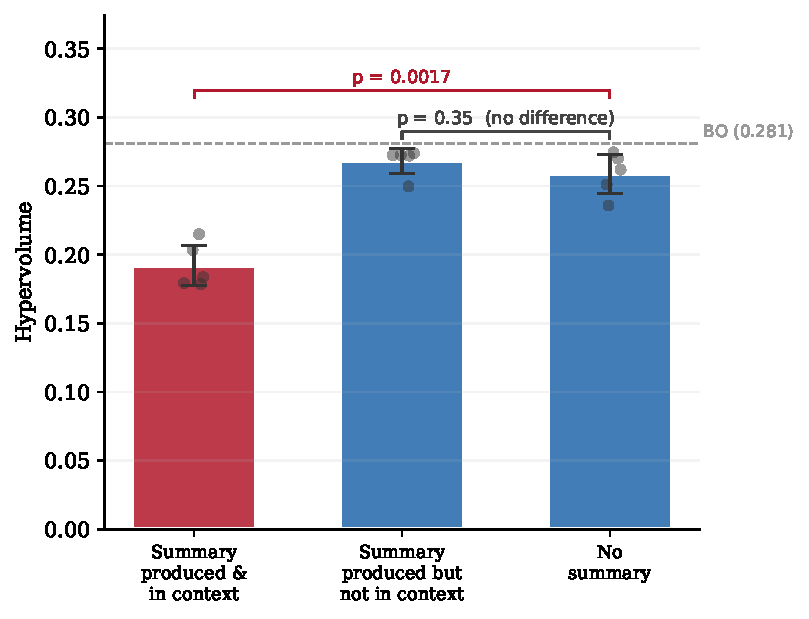
\includegraphics[width=0.55\textwidth]{fig6_mechanism_isolation.pdf}
\caption{Mechanism isolation on \baseline{} (Opus, $n = 5$, seeds
  42--46). The summary-not-fed condition (produced but not persisted
  in context) performs identically to no summary (\pval{0.35}). Both
  significantly outperform full VR (\pval{0.002}). Dashed line: BO
  reference. The act of articulation is free; persistence is costly.}
\label{fig:mechanism}
\end{figure}

The summary-not-fed condition performs identically to the no-summary
condition (paired $t$-test, \pval{0.35}) and significantly outperforms
the full VR condition (\pval{0.002}). The act of producing the structured
summary---including the LLM call, the token cost, and the cognitive work
of articulation---has zero measurable effect on optimization quality.
The entire performance gap comes from \emph{persisting} the summary in the
conversation context, where it cements early beliefs (including
incorrect ones such as dismissing $X_5 \to Y_2$ at confidence~0.1) into
subsequent iterations.

\FloatBarrier
\subsection{Discovery decouples from exploitation below Sonnet tier}
\label{sec:model_gradient}

We run three models on \noisy{} at 72 evaluations ($n = 3$ seeds each):
Opus~4.6, Sonnet~4.6, and Haiku~4.5. \Cref{fig:model_gradient} shows
the results.

\begin{figure}[htbp]
\centering
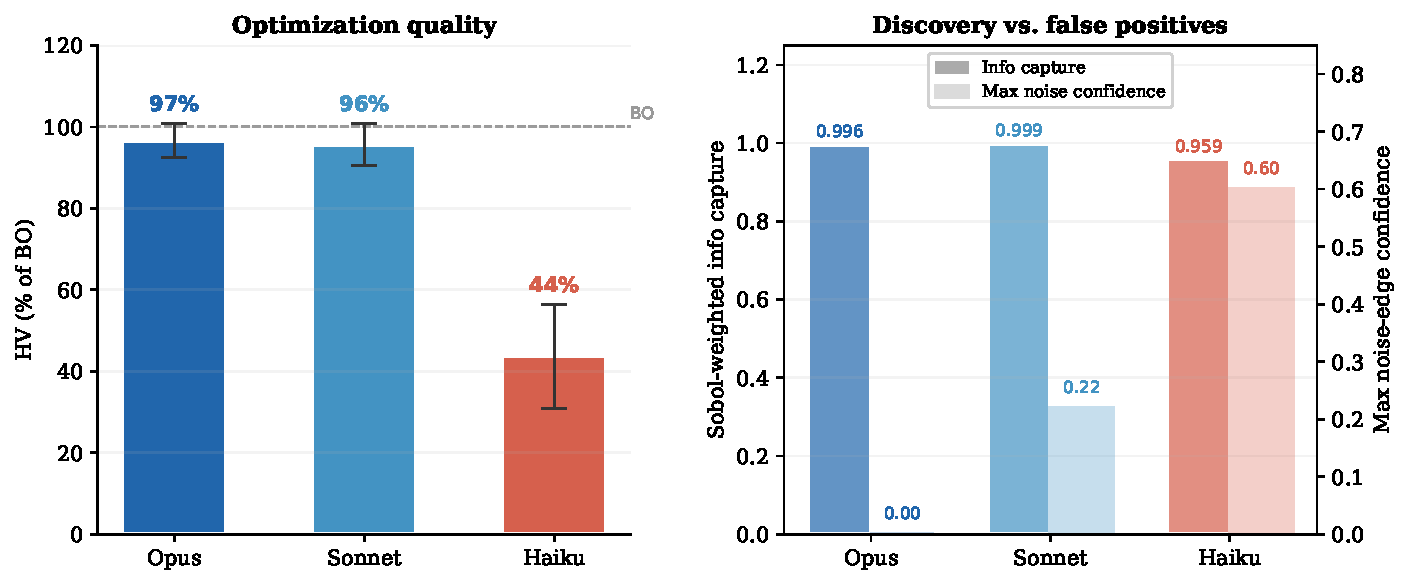
\includegraphics[width=\textwidth]{fig7_model_gradient.pdf}
\caption{Model capability gradient on \noisy{} (72 evaluations,
  $n = 3$ seeds each). Left: HV as percentage of BO. Opus and Sonnet
  achieve near-parity (${\geq}96\%$); Haiku collapses to 44\%. Right:
  Sobol-weighted information capture (solid bars) vs.\ maximum
  noise-edge confidence (hatched bars). Haiku discovers the correct
  causal structure (info capture 0.96) but cannot exploit it and
  generates false-positive noise edges.}
\label{fig:model_gradient}
\end{figure}

Opus and Sonnet achieve near-parity with BO (97\% and 96\%
respectively) and maintain perfect edge precision---zero false-positive
noise edges, with the highest confidence assigned to any noise-input
edge at $\leq 0.22$ out of~1.0, indicating clear dismissal. The two
models
achieve similar outcomes via different cognitive strategies: Opus
dismisses noise inputs by inference alone (0\% of OAT sweeps on noise
dimensions), while Sonnet verifies empirically (20\% noise OAT sweeps)
before dismissing.

At Haiku tier, a qualitative break occurs. HV drops to 44\% of BO, and
the agent claims two noise edges at confidence 0.55 and 0.60---the only
false positives in the entire experimental suite. Yet Haiku's
Sobol-weighted information capture remains 0.96---near parity with
Opus and Sonnet. Haiku \emph{discovers} the correct causal structure but
cannot \emph{exploit} it for optimization and cannot reliably distinguish
real from spurious edges. This discovery--exploitation decoupling
suggests the two capabilities have different model-capability thresholds.

% ══════════════════════════════════════════════════════════════════
\FloatBarrier
\section{Discussion}
\label{sec:discussion}

\subsection{The concept bottleneck interpretation}

The structured iteration summary functions as a learned concept
bottleneck (\cref{sec:related}): an interpretable intermediate
representation that mediates between observations and decisions. Our
$2 \times 2$ matrix empirically confirms the prediction from the CBM
literature: bottlenecks help when concepts are correct and hurt when
they are wrong. On \noisy{}, the agent's early belief that noise
dimensions are irrelevant is correct, and persisting this belief via the
summary provides useful scaffolding. On \baseline{}, the agent's early
belief that $X_5$ has weak influence (dismissed at confidence~0.1) is
wrong---$X_5$ drives a hidden threshold mechanism---and persisting this
incorrect belief cements the error.

A key difference from standard CBMs is that our bottleneck is
\emph{discovered}, not designed. In a CBM, the researcher specifies
which concepts to include; if they choose wrong, performance suffers.
In our setting, the agent constructs its own concepts (causal edges with
confidence scores), and the quality of this construction depends on the
agent's capability and the task's difficulty. This makes the
scaffolding--regularization distinction model-dependent: the same
protocol is scaffolding for one model and an impediment for another.

\subsection{Ephemeral versus persistent reasoning traces}

Our finding that the \emph{persistence} of reasoning traces---not their
production---drives the performance penalty raises a natural question
about multi-turn LLM agent design more broadly: should reasoning
artifacts be carried forward across turns, or treated as ephemeral?
Recent reasoning-oriented models architecturally separate reasoning
traces from conversation context---producing extended chain-of-thought
tokens that are not presented to the user and may not persist verbatim
into subsequent turns. Our three-condition ablation provides one
controlled data point: in our setting, ephemerality is strictly better
than persistence when the persisted content contains early-stage causal
beliefs. Whether this extends to other forms of persistent reasoning
(e.g., maintained plans, accumulated observations) is untested.

\subsection{Design principles}

Our results suggest three practical guidelines for practitioners building
LLM optimization agents:

\begin{enumerate}
  \item \textbf{Match protocol rigidity to the capability gap.} Use
  structured summaries when the model needs help organizing its
  reasoning (less capable models, higher-dimensional tasks). Omit them
  when the model can effectively reason without imposed structure.

  \item \textbf{Prefer ephemeral over persistent reasoning traces.}
  If structured articulation is used for interpretability or logging,
  consider not feeding the summary back into the agent's context. Our
  mechanism-isolation experiment shows this preserves all the benefit
  of articulation (the summary is still produced and logged) while
  avoiding context cementing.

  \item \textbf{There is a model capability floor for reliable causal
  reasoning.} Below a sufficient capability threshold (between
  Sonnet~4.6 and Haiku~4.5 in our experiments), causal discovery
  decouples from exploitation: the agent identifies structure but
  cannot use it effectively and may generate false-positive claims.
\end{enumerate}

\subsection{Limitations}

\paragraph{Synthetic oracles only.} SynthOracle's functional forms are
deterministic, noise-free, and low-dimensional relative to real
scientific systems. Whether the scaffolding finding transfers to
stochastic, high-dimensional physical simulators remains untested.

\paragraph{Single reasoning protocol.} We evaluate one VR protocol
design. Alternative structured-reasoning approaches (BORA's adaptive
policy, ReAct-style interleaving, simple free-text reflection) were not
compared. Our finding is about the effect of \emph{persisting} structured
summaries, not about the specific VR protocol being optimal.

\paragraph{Sample sizes.} Most conditions use $n = 5$ seeds. Only one
of four cells in the $2 \times 2$ matrix reaches individual significance
at $p < 0.05$ (Opus $\times$ \baseline{}, \pval{0.0006}); the others
are directional but underpowered ($p = 0.054$, $0.095$, $0.169$). Our
primary statistical claim rests on the global sign test: 18 of 20 paired
seeds follow the scaffolding prediction (binomial \pval{0.0002}). This
tests the \emph{pattern}---one cell hurts, three help---rather than
individual cell significance. Additional seeds would tighten per-cell
confidence intervals but the directional pattern is already robust.
We pre-registered predictions for four experimental conditions before
running them; three of four were qualitatively wrong
(\cref{app:preregistration}), underscoring the value of controlled
ablation over intuition.

\paragraph{Articulation format.} The scaffolding effect may depend on
\emph{what} is articulated. Our protocol requires causal edges with
confidence scores---a specific, structured format that cements specific
beliefs. A protocol that articulated optimization priorities,
uncertainty estimates, or free-text reflections instead might show
different cell-by-cell effects. The finding that persistence hurts is
likely general; the specific interaction with model capability and task
difficulty may be format-dependent.

% ══════════════════════════════════════════════════════════════════
\section{Conclusion}
\label{sec:conclusion}

We introduced SynthOracle, a benchmark with ground-truth causal
structure that enables separate measurement of optimization quality and
reasoning quality in LLM agents. Using this benchmark, we tested the
assumption that forcing LLM agents to articulate structured reasoning
regularizes their behavior---and found it wrong in general.

The forced structured summary is scaffolding, not regularization. It
helps agents that need structure (less capable models, harder tasks with
irrelevant dimensions) and hurts the most capable model on the simplest
task. The mechanism is context cementing: persisting the summary in
conversation context anchors early beliefs into subsequent iterations.
The act of articulation itself is free---an agent that produces the
summary but does not receive it back performs identically to one that
never produces it.

This finding has a direct practical implication: when building LLM
optimization agents, match the rigidity of your reasoning protocol to
the gap between your model's capability and your task's difficulty. And
if you use structured summaries for interpretability, consider making
them ephemeral rather than persistent---you keep the logging benefit
without the cementing cost.

More broadly, the context-cementing mechanism suggests that how LLM
agents \emph{remember} their reasoning matters as much as whether they
reason at all. The architectural trend toward ephemeral chain-of-thought
in frontier reasoning models is consistent with this principle. Our
benchmark provides a controlled setting for future work on reasoning
persistence, belief revision, and the conditions under which structured
articulation helps versus harms autonomous scientific agents.


\begin{thebibliography}{10}

\bibitem{cisse2025bora}
K.~Cisse, Y.~Shi, and S.~Zhe.
\newblock BORA: A modular {LLM}-based adaptive {B}ayesian optimization
  research agent.
\newblock In \emph{Proc.\ IJCAI}, 2025.

\bibitem{boiko2023autonomous}
D.~A.~Boiko, R.~MacKnight, and G.~Gomes.
\newblock Autonomous chemical research with large language models.
\newblock \emph{Nature}, 624:570--578, 2023.

\bibitem{ramos2024bayesian}
M.~Acosta~Ramos, P.~A.~Ortega, et~al.
\newblock Bayesian optimization with {LLM} surrogates.
\newblock \emph{arXiv preprint}, 2024.

\bibitem{chi1994selfexplanation}
M.~T.~H.~Chi, N.~de~Leeuw, M.-H.~Chiu, and C.~LaVancher.
\newblock Eliciting self-explanations improves understanding.
\newblock \emph{Cognitive Science}, 18(3):439--477, 1994.

\bibitem{gupta2025arewethereyet}
A.~Gupta, Y.~Du, A.~Nair, P.~Agrawal, and F.~Sala.
\newblock Are we there yet? {A} critical analysis of {LLM} agents in
  closed-loop experimental design.
\newblock \emph{arXiv:2503.15547}, 2025.

\bibitem{koh2020cbm}
P.~W.~Koh, T.~Nguyen, Y.~S.~Tang, S.~Mussmann, E.~Pierson, B.~Kim, and
  P.~Liang.
\newblock Concept bottleneck models.
\newblock In \emph{Proc.\ ICML}, pp.~5338--5348, 2020.

\bibitem{yuksekgonul2023posthoc}
M.~Y\"{u}ksekgon\"{u}l, M.~Wang, and J.~Zou.
\newblock Post-hoc concept bottleneck models.
\newblock In \emph{Proc.\ ICLR}, 2023.

\bibitem{wei2022chainofthought}
J.~Wei, X.~Wang, D.~Schuurmans, M.~Bosma, B.~Ichter, F.~Xia, E.~Chi,
  Q.~V.~Le, and D.~Zhou.
\newblock Chain-of-thought prompting elicits reasoning in large language models.
\newblock In \emph{Advances in NeurIPS}, 2022.

\bibitem{yao2023react}
S.~Yao, J.~Zhao, D.~Yu, N.~Du, I.~Shafran, K.~Narasimhan, and Y.~Cao.
\newblock {ReAct}: Synergizing reasoning and acting in language models.
\newblock In \emph{Proc.\ ICLR}, 2023.

\bibitem{daulton2021nehvi}
S.~Daulton, M.~Balandat, and E.~Bakshy.
\newblock Parallel {B}ayesian optimization of multiple noisy objectives with
  expected hypervolume improvement.
\newblock In \emph{Advances in NeurIPS}, 2021.

\end{thebibliography}

% ══════════════════════════════════════════════════════════════════
\clearpage
\appendix

\section{Oracle Specifications}
\label{app:oracle_specs}

All oracles map inputs $X_i \in [0.1, 1.0]$ to four outputs with
directions: maximize~$Y_1$, minimize~$Y_2$, threshold~$Y_3 > 0.4$,
maximize~$Y_4$. We use $\sigma(x) = 1/(1 + e^{-x})$ throughout.

\subsection{\baseline{} (reference)}

\textbf{Mechanisms:}
\begin{align*}
  M_1 &= X_2^{1.37} \cdot X_4^{0.82} \cdot (1 - e^{-5X_1})
    & &\text{(throughput)} \\
  M_2 &= 0.55 \cdot e^{-1.8 X_3 \sqrt{X_1}}
    & &\text{(leakage)} \\
  M_3 &= X_4 / (X_4 + X_6)
    & &\text{(coupling)} \\
  g &= \sigma(25(X_5 - 0.38))
    & &\text{(threshold gate)}
\end{align*}

\textbf{Effective mechanisms:}
\begin{align*}
  M_1^{\text{eff}} &= M_1 \cdot M_3 &
  M_2^{\text{eff}} &= M_2 \cdot (1 - 0.6 M_3) \\
  M_4^{\times} &= 1 + 0.4 X_6 \cdot g &
  M_4^{+} &= 0.5 X_6 \cdot g
\end{align*}

\textbf{Outputs:}
\begin{align*}
  Y_1 &= M_1^{\text{eff}} \cdot M_4^{\times} + M_4^{+}
         - M_2^{\text{eff}} \\
  Y_2 &= 0.85 M_2^{\text{eff}}
         + 0.35 M_1^{\text{eff}} / M_4^{\times}
         + 0.25(1 - M_3) \\
  Y_3 &= \sigma(8.1(X_1 - 0.27)) \cdot X_3^{0.5} \\
  Y_4 &= M_1^{\text{eff}} / (1 + 2 M_1^{\text{eff}})
\end{align*}

\subsection{\shifted{} (functional forms altered)}

Same mechanism topology as \baseline{} with the following changes:
\begin{itemize}
  \item Coupling weakened: $M_3 = X_4 / (X_4 + 0.5 X_6)$
  \item Threshold disabled: $g \equiv 1$
  \item $Y_1$: adds smooth $X_5$ contribution ($0.3 X_5^{0.8}$) and
    $X_1 \times X_5$ interaction ($0.8 X_1 X_5$)
  \item $Y_2$: $M_1^{\text{eff}}$ sign flipped ($-0.20$ instead of
    $+0.35$); adds $X_5$ penalty ($0.15 X_5$)
  \item $Y_3$: inverted-U in $X_3$ (peaks at $X_3 \approx 0.6$)
    instead of $X_3^{0.5}$
  \item $Y_4$: adds log contribution ($0.12 \ln(1 + 3X_3)$); weaker
    saturation ($1.5$ instead of $2.0$)
\end{itemize}

\subsection{\rewired{} (input--mechanism wiring swapped)}

Same functional forms as \baseline{}, but with input assignments
permuted:
\begin{itemize}
  \item $M_1$: $X_3^{1.37} \cdot X_6^{0.82} \cdot (1 - e^{-5X_1})$
    \quad (was $X_2, X_4$)
  \item $M_2$: $0.55 \cdot e^{-1.8 X_4 \sqrt{X_1}}$
    \quad (was $X_3$)
  \item $M_3$: $X_2 / (X_2 + X_5)$
    \quad (was $X_4, X_6$)
  \item Gate: $\sigma(25(X_6 - 0.38))$
    \quad (was $X_5$)
  \item $M_4$: uses $X_5 \cdot g(X_6)$
    \quad (was $X_6 \cdot g(X_5)$)
  \item $Y_3$: $\sigma(8.1(X_1 - 0.27)) \cdot X_4^{0.5}$
    \quad (was $X_3$)
\end{itemize}

\subsection{\noisy{} (12-dimensional)}

Identical to \baseline{} for inputs $X_1$--$X_6$. Inputs
$X_7$--$X_{12}$ have zero effect on all outputs. The oracle wraps
\baseline{} and passes only $X_1$--$X_6$ to the inner evaluation
function.

% ══════════════════════════════════════════════════════════════════
\section{VR Prompt and Output Schema}
\label{app:prompt}

The agent receives a system prompt at the start of each run containing:
(1)~the oracle's input names and bounds, (2)~output names and
optimization directions, (3)~the constraint $Y_3 > 0.4$, and (4)~a
description of the hypothesize--predict--reconcile loop. No information
about the underlying mechanism structure is provided. A representative
excerpt:

\begin{quote}\small
\emph{You are optimizing a system with 6 inputs ($X_1$--$X_6$, each in
$[0.1, 1.0]$) and 4 outputs: maximize $Y_1$, minimize $Y_2$, ensure
$Y_3 > 0.4$, maximize $Y_4$. You have a budget of 72 oracle
evaluations. Before each evaluation, predict the output values. After
observing results, update your causal model. Use OAT sweeps to
understand input--output relationships and interaction tests to detect
coupling. Your goal is to find the Pareto-optimal trade-off while
building a causal understanding of the system.}
\end{quote}

At the end of each iteration, the agent's output is parsed against a
fixed schema requiring: a list of causal edges (source, target,
confidence 0--1, rationale), surprise observations, new findings, and a
plan for the next iteration. The full prompt text and schema definition
are available in the code repository.

% ══════════════════════════════════════════════════════════════════
\section{Edge Detection Threshold Sensitivity}
\label{app:threshold_sensitivity}

\Cref{tab:threshold} shows edge precision and recall as a function of the
detection threshold, computed across all OAT sweeps in the \baseline{}
and \noisy{} 72-evaluation runs ($n = 5$ seeds each). When a real input
is varied in an OAT sweep, the output changes by 0.006 to 0.666
(depending on the edge strength and base point). When a noise input is
varied, the output change is exactly 0.000. The complete separation means precision is 1.00 at all
tested thresholds. We report results at 0.05 as a conservative default.

\begin{table}[h]
\centering
\caption{Edge precision and recall vs.\ detection threshold.}
\label{tab:threshold}
\small
\begin{tabular}{@{}ccccc@{}}
\toprule
Threshold & Precision & Recall & TP & FN \\
\midrule
0.01 & 1.000 & 0.948 & 147 & 8 \\
0.02 & 1.000 & 0.948 & 147 & 8 \\
0.03 & 1.000 & 0.948 & 147 & 8 \\
0.05 & 1.000 & 0.935 & 145 & 10 \\
0.10 & 1.000 & 0.710 & 110 & 45 \\
0.15 & 1.000 & 0.619 & 96 & 59 \\
0.20 & 1.000 & 0.503 & 78 & 77 \\
\bottomrule
\end{tabular}
\end{table}

% ══════════════════════════════════════════════════════════════════
\section{Additional Diagnostics}
\label{app:additional_diagnostics}

The following metrics are available in the SynthOracle benchmark but are
not central to the main paper's claims. We report them here for
completeness.

\paragraph{Sobol-weighted information capture.} Weights each
input--output edge by its Sobol total-effect index, measuring whether
the agent discovers the \emph{high-impact} edges. Across all conditions,
information capture exceeds 0.96, indicating the agent consistently
identifies the most important causal relationships even when raw recall
is lower (e.g., \noisy{} at 72 evaluations: recall = 0.70, info capture
= 0.996).

\paragraph{OAT prediction accuracy.} Before each OAT sweep, the agent
predicts whether each output will increase or decrease as the swept
input varies. Direction accuracy---the fraction of correct
increase/decrease predictions---ranges from 66\% (Haiku) to 91\%
(\noisy{} Opus at 72 evaluations), against a 50\% random baseline.

\paragraph{Sample efficiency.} The number of evaluations required to
reach 50\%, 75\%, and 90\% of reference hypervolume. On \baseline{}, VR
requires 20--30 evaluations for 50\% (vs.\ 10 for BO) and 50--60
evaluations for 75\% (vs.\ 26 for BO). The gap narrows at higher
thresholds, reflecting VR's front-loaded investment in model building.

\paragraph{Adversarial region error.} Prediction MAE in ``hard''
regions (near coupling boundaries, threshold transitions) versus
``easy'' regions. On \noisy{} at 144 evaluations, adversarial MAE
drops 60--67\% from 72 to 144 evaluations, indicating the agent
progressively learns difficult regions.

% ══════════════════════════════════════════════════════════════════
\section{Transfer Results}
\label{app:transfer}

We tested whether a causal model learned on \baseline{} transfers to
\shifted{} (same topology, altered functional forms) and \rewired{}
(altered topology). The agent receives the prior causal model in its
initial prompt and uses a screen-first protocol: it empirically tests
each claimed edge before committing to prior beliefs.

\begin{table}[h]
\centering
\caption{Transfer results (Opus, 72 evaluations, $n = 3$ seeds
  42--44). Effect: prior HV minus fresh HV as percentage of fresh.}
\label{tab:transfer}
\small
\begin{tabular}{@{}lccccc@{}}
\toprule
Oracle & Prior HV & Fresh HV & Effect & $p$ & Dir.\ \\
\midrule
\shifted{}  & $1.209 \pm .120$ & $1.186 \pm .074$ & $+2\%$ & 0.751 & 2/3 \\
\rewired{}  & $0.272 \pm .005$ & $0.260 \pm .011$ & $+5\%$ & 0.246 & 3/3 \\
\bottomrule
\end{tabular}
\end{table}

Both comparisons are directionally positive (prior helps) but not
statistically significant at $n = 3$. The \shifted{} result is
particularly noisy: seed~42 shows the prior \emph{hurting} ($-10\%$),
while seeds 43 and 44 show modest benefit. The \rewired{} result is
more consistent (3/3 positive) but the effect is small. We report these
as directional observations requiring larger sample sizes to confirm.

% ══════════════════════════════════════════════════════════════════
\section{Pre-Registered Predictions}
\label{app:preregistration}

Before running the gap-closing experiments, we committed predictions for
four experimental conditions. Three of four were qualitatively wrong.

\begin{table}[h]
\centering
\caption{Pre-registered predictions vs.\ actual outcomes.}
\label{tab:preregistration}
\small
\begin{tabular}{@{}p{3cm}p{3cm}p{3cm}p{4cm}@{}}
\toprule
Prediction & Expected & Actual & Why we were wrong \\
\midrule
$R^2(M \!\to\! Y)$ predicts VR/BO
  & Low $R^2$ $\to$ worse VR
  & Low-$R^2$ oracles have \emph{higher} VR/BO
  & $R^2$ measures mechanism interpretability, not optimization difficulty; BO also struggles on low-$R^2$ oracles \\[4pt]
Wrong prior hurts on \shifted{}
  & $-9\%$ penalty
  & $+2\%$ (prior helps)
  & Screen-first protocol filters incorrect prior edges; partial correct structure still provides value \\[4pt]
VR crosses BO at extended budget
  & VR $>$ BO at 144
  & VR $= 99\%$ of BO
  & Assumed BO was saturated at 72 evals; it was not (BO also improves with more budget) \\[4pt]
Sonnet replicates Opus on \noisy{}
  & Same HV and strategy
  & HV matches; strategy differs
  & Correct on outcome; did not predict that Sonnet would verify noise empirically rather than dismiss by inference \\
\bottomrule
\end{tabular}
\end{table}

\end{document}
